\documentclass[conference]{IEEEtran}
\usepackage{threeparttable}
\usepackage{color}
\usepackage{amsmath}
\usepackage{graphicx}
\usepackage{epstopdf}
%************ COMMENT BELOW WHEN NOT NEEDED ************%
%\usepackage{zref-totpages}
%\AtBeginDocument{
  %%\ifnum\ztotpages>6 %
    %\hypersetup{pdfstartpage=3,
		%%colorlinks = true, %Colors links instead of ugly boxes
		%%urlcolor = blue, %Color for external hyperlinks
		%%linkcolor = blue, %Color of internal links
		%%citecolor = red,  %Color of citations
		%}%
%%	\else
%%		\hypersetup{pdfstartpage=5}%
  %%\fi
%}
%\usepackage[pdftex,hidelinks]{hyperref}
%\usepackage{titlesec}
%\usepackage{indentfirst}
%************ END COMMENT ABOVE WHEN NOT NEEDED ************%
\newcommand{\rmnum}[1]{\romannumeral #1}
\newcommand{\Rmnum}[1]{\MakeUppercase{\romannumeral #1}}
\newcommand{\vect}[1]{\overline {#1}}
\newcommand{\vm}[1]{{\bf{#1}}}
\newcommand{\argmin}{\operatornamewithlimits{argmin}}
\newcommand{\argmax}{\operatornamewithlimits{argmax}}
\newcommand{\idxmin}{\operatornamewithlimits{idxmin}}
\newcommand{\idxmax}{\operatornamewithlimits{idxmax}}
\newcommand{\twopartdef}[4]
{
	\left\{
		\begin{array}{ll}
			#1 &; #2 \\
			#3 &; #4
		\end{array}
	\right.
}
\newcommand{\vecttwo}[2]
{
	\left[
		\begin{IEEEeqnarraybox*}[][c]{c}
		#1\\
		#2
		\end{IEEEeqnarraybox*}
	\right]
}
\newcommand{\vectthree}[3]
{
	\left[
		\begin{IEEEeqnarraybox*}[][c]{c}
		#1\\
		#2\\
		#3
		\end{IEEEeqnarraybox*}
	\right]
}
\begin{document}
\bstctlcite{IEEEexample:BSTcontrol}
% 
% paper title
% can use linebreaks \\ within to get better formatting as desired
\title{Multi-Wavelength Visible Light Communication System Design}


% author names and affiliations
% use a multiple column layout for up to two different
% affiliations

\author{\IEEEauthorblockN{Pankil M. Butala, Hany Elgala, Thomas D.C. Little}
\IEEEauthorblockA{Department of Electrical and Computer Engineering\\
Boston University, Boston, MA, USA\\
\{pbutala, helgala, tdcl\}@bu.edu}
 %Payman Zarkesh-Ha, Thomas D.C. Little}
\and
\IEEEauthorblockN{Payman Zarkesh-Ha}
\IEEEauthorblockA{Department of Electrical and Computer Engineering\\
University of New Mexico, Albuquerque, NM, USA\\
payman@ece.unm.edu}}

% make the title area
\maketitle

Visible light communications (VLC) are achieved by modulation of one or more spectral components in the visible spectrum ($\approx$400-800 nm). The use of this range provides an opportunity to exploit an otherwise untapped medium that is used in human lighting. Most visible light communication systems constructed to date focus on using a broad visible band generated by phosphor-converted blue light emitting diodes, or by filtering to isolate the blue components from these sources. Multi-wavelength systems consider multiple wavelength bands that are combined to produce the desired spectrum realizing a desired color temperature and intensity. The use of multiple bands is also a form of wavelength-division multiplexing. In this paper, we investigate the relationships between the colors comprising the lighting source for a range of lighting states, the spectral separation of communication channels, the relative intensities required to realize lighting states, how modulation can be most effectively mapped to the available color channels, and the design of an optical filtering approach to maximize SNR while minimizing crosstalk at the receiver. Simulation results based on a three colored VLC system are discussed using orthogonal frequency division multiplexing for each color. We show that the system is the most power efficient at 6250 K correlated color temperature, with transmitter spectral spread of 5 nm and filter transmittance width of 40 nm.

\begin{IEEEkeywords}
Visible Light Communications (VLC), Optical Wireless Communications (OWC), Multiple Input Multiple Output (MIMO), Wavelength Division Multiplexing (WDM), Orthogonal Frequency Division Multiplexing (OFDM).
\end{IEEEkeywords}

\IEEEpeerreviewmaketitle
% introduction
\section{Introduction}
%Spectrum crunch. Solid state lighting wave. VLC as a means to mitigate downlink bottleneck.\\
%Smart spaces.  Multi-colored LEDs. Color tunability + WDM.\\
%ACO-OFDM. DCO-OFDM. O-OFDM background.\\
%In this work, find optimal range of operation for communication.
%O-OFDM over each color WDM + O-OFDM. More capacity.\\
There has been a rapid increase in use of networked portable computing devices in recent years. These devices are consuming increasingly more information in the form of multimedia streaming \cite{cis14a}. Trying to keep up with this increasing demand for wireless data has strained the network infrastructure thus creating the phenomenon of 'spectrum crunch'. Its effect can be seen in reduced quality of service and lower download speeds. 

On the other hand, advances made by the solid state industry has created energy efficient illumination devices called light emitting diodes (LED). The intensity of radiant flux emitted by LEDs can be modulated at a high enough rate such that information transfer can be achieved at relatively high speeds while the intensity variations are invisible to human eye. One or more LEDs can be packaged together to form a 'luminaire' which under the above model services the dual functionality of providing wireless network access and maintaining illumination \cite{kom04a}. The additional downlink capacity provided by such ``smart'' luminaires can help mitigate some of the aforementioned spectrum crunch.

A simple single input single output visible light communications (VLC) channel can be created by using an LED as a transmitter and a photodiode as a receiver. Channel characteristics for an optical channel are described in reference \cite{kah97a}. Another way of improving the capacity of a wireless channel is by using multiple transmitting and receiving elements in a multiple input multiple output (MIMO) configuration. Different types of MIMO systems \cite{hra06a,zen09a,ash10a,but13a,but14b} have been reported in literature.

One type of an optical MIMO system is wavelength division multiplexed (WDM) VLC system. Different WDM system prototypes have been reported in literature \cite{wan11a,kot12a,cos12a}. These describe an instance of a WDM system without analysis of the optimal operating point. In this work, design of multi-wavelength VLC systems under lighting constraints when correlated color temperature (CCT) of illumination, transmitter spectral power distribution (SPD) and receivers' filter spectral transmittance full width at half maximum (FWHM) are varied, is studied for the first time. Simulations for a three colored WDM VLC system then provide numerical analysis of the system performance giving an insight into optimal design criteria. For the system considered, we find that its most power efficient operation occurs at CCT of 6250 K, narrow transmitting elements' SPD (5 nm), and receiver filter FWHM of 40 nm.

The following notations are used in this paper. Scalar values are represented in regular font. Vectors and matrices are represented in bold font. Conjugate transpose of $\vm{A}$ is represented by $\vm{A}^{*}$. Operators $:=$ and $||.||$ represent definition and euclidean norm respectively. 

An introduction to optical MIMO systems is provided in Section \ref{sec:mimo}. WDM, a subset of optical MIMO systems, is introduced in Section \ref{sec:wdm}. Section \ref{sec:simulation} describes the simulation setup. Results and discussion is provided in Section \ref{sec:results}. Conclusions are then drawn in Section \ref{sec:conclusion}. 
% MIMO Channel Matrix
\section{Optical MIMO Channel}\label{sec:mimo}
This section provides an introduction to an optical MIMO channel that can be established between multiple optical transmitting and receiving elements. Information over an optical channel is usually transmitted using intensity-modulation direct-detection (IM/DD). At the transmitting elements, information is modulated over the intensity of emitted light or radiant flux. Since output light intensity from a radiating source must be non-negative, the transmitted signals must be constrained to non-negative values. Multiple transmitting elements can be established over dimensions such as space, time, frequency, wavelength, polarization, and others. Each receiving element must produce an output electrical signal that is proportional to the radiant flux, from the dimension of interest, incident on it. Each parallel link must be sufficiently decorrelated with enough signal to interference and noise ratio (SINR) to meet the target bit error rate (BER). 

A typical optical MIMO channel can be modeled as a linear time invariant system and be represented as
\begin{equation}
	\label{eqMIMOch}
	\vm{Y} = \vm{H}\vm{X} + \vm{W}
\end{equation}
$\vm{X}$ is an $N_{tx}$ dimensional vector. Each element of $\vm{X}$ represents the radiant flux emitted by each transmitting element. $\vm{Y}$ is an $N_{rx}$ dimensional vector. Each element of $\vm{Y}$ represents the signal output from each receiving element. $\vm{H}$ is an $N_{rx}\times N_{tx}$ dimensional channel matrix. Each element $h_{ij}\in \vm{H};$ $i\in \{1,2,\dots, N_{rx}\},$ $j\in \{1,2,\dots, N_{tx}\}$ represents the conversion factor for signal output from the $i^{th}$ receiving element when radiant flux from $j^{th}$ transmitting element is incident on it after including the path losses. $\vm{W}$ is an $N_{rx}$ dimensional noise vector. It is typically modeled as additive white Gaussian noise independent of transmitted vector $\vm{X}$ i.e. $\vm{W}\sim\mathcal{N}({\bf{0}},\sigma_n^2\vm{I}_{N_{rx}})$.

The amount of radiant flux per solid angle emitted by the $j^{th}$ transmitting element in a certain angular direction $\phi$ is given by the angular radiant intensity distribution. An LED's radiant intensity distribution is usually characterized by a Lambertian distribution given by
\begin{equation}
	\label{eqLamb}
	L_j(m,\phi) = \twopartdef{{\frac{(m+1)}{2\pi}}cos^{m}(\phi)}{-\pi/2\leq\phi\leq\pi/2}{0}{\mbox{ else}}
\end{equation}
If $\Phi$ is the emission angle at which radiant intensity of a transmitting element is half its peak value (at $\psi=0^\circ$), the Lambertian order of that emission is $m=-ln(2)/ln(cos(\Phi_{j}))$.

A photodiode is a device that produces an electrical signal output that is proportional to the radiant flux incident on it. Photodiodes with larger active area can collect greater flux and thus output a larger signal. On the other hand, a large area photodiode offers a larger capacitance and thus reduces the signal bandwidth that can be received without distortion. Additionally, this also reduces the number of photodiodes that can be packed together to form a multi-element receiving array within a given area budget on a portable device. The photodiode effective area can be increased by using optics. Concentrator optics may be used for each photodiode element in non-imaging receiver arrays. The area gain provided by concentrator optics on the $i^{th}$ receiving element is given by
\begin{equation}
	\label{eqGain}
	G_i(\psi) = \twopartdef{\frac{\eta_i^2}{sin^2(\Psi_{i})}} {0\leq\psi\leq\Psi_{i}\leq\frac{\pi}{2}}{0}{\psi>\Psi_{i}}
\end{equation}
where $\psi$ is the angle of incidence of the incident flux, $\eta$ is the refractive index of the material that the optics are made of, and $\Psi_i$ is the field of view of the $i^{th}$ concentrator.

Optical filters may be used at the receiver to acquire only the wavelengths of interest while rejecting the ambient radiation. Depending on the type of filter used, its transmittance may be a function of the angle of incidence $\psi$. Let $T_i(\psi,\lambda)$ be the transmittance of the $i^{th}$ optical filter. If $S(\lambda)$ is the normalized spectral power distribution (SPD) of incident radiation and $R_i(\lambda)$ is the responsivity of the $i_{th}$ receiving photodiode, the effective responsivity of the $i^{th}$ receiving element is given by
\begin{equation}
	\label{eqReff}
	R_{e_i}(\psi) = G_i(\psi)\int^{\lambda_{max}}_{\lambda_{min}}S(\lambda)T_i(\psi,\lambda)R_i(\lambda)d\lambda
\end{equation}

Let $\vm{d}_{ij}$ be the vector from receiving element $i$ to transmitting element $j$. The distance between the two is then given by $||\vm{d}_{ij}||^2$. Let $A_i$ be the active area of the photodiode. The channel gain from transmitting element $j$ to receiving element $i$ is given by
\begin{equation}
	\label{eqChGain}
	h_{ij} = L_{m_j}(\phi_{ij})\frac{A_i}{||\vm{d}_{ij}||^{2}}cos(\psi_{ij})R_{e_i}(\psi_{ij})
\end{equation}
where $m_j$ is the Lambertian order of the $j^{th}$ transmitting element, and $\phi_{ij}$ and $\psi_{ij}$ are the angles subtended between vector $\vm{d}_{ij}$ and surface normals respectively of the $j^{th}$ transmitting and $i^{th}$ receiving elements.

Ambient light incident on a photodiode generates shot noise. Let $P_a(\lambda)$ be SPD of isotropic ambient light. This would generate shot noise in the $i^{th}$ receiving element with variance
\begin{equation}
	\label{eqNshot}
	\sigma_{sh_i}^{2} = \frac{2qA_iG_i(\Psi_i)}{\Psi_i}\int_{\lambda_{min}}^{\lambda_{max}}\int_{0}^{\Psi_i}P_{a}(\lambda)T_i(\psi,\lambda)R_i(\lambda)d\psi d\lambda
\end{equation}
where $q=1.6\times 10^{-19}$ C is the charge of an electron. Shot noise statistics are typically modeled as a Poisson distribution. 

A trans-impedance amplifier (TIA) is most often used as the first stage amplifier. Thermal noise is the most dominant component of TIA electrical noise. The thermal noise variance in the $i^{th}$ receiving element is given by
\begin{equation}
	\label{eqNth}
	\sigma_{th_i}^{2} = \frac{4kT_i}{R_{f_i}}
\end{equation}
where constant $k$ is Boltzmann constant, $T_i$ is the absolute temperature and $R_{f_i}$ is the TIA feedback resistance. Thermal noise statistics are typically modeled as a Gaussian distribution.

Total input referred noise variance is usually approximated as the sum of shot noise variance and thermal noise variance.  For sake of mathematical simplicity, total noise is assumed to have Gaussian statistics with mean $0$ and variance $\sigma_{n_i}^{2} = \sigma_{sh_i}^{2} + \sigma_{th_i}^{2}$.

In VLC, transmitting elements perform dual function of providing wireless data transmission while maintaining illumination levels. To perform a fair comparison between different modulation systems operating at same illumination levels needs a different definition of SNR. In this work, SNR is defined as the ratio of the average transmitted electrical power to noise power and is similar as in \cite{fat13a}. 
\begin{equation}
	\label{eqSNR}
	SNR^{tx}_{avg} = \frac{(hP_{avg}^{tx})^2}{\sigma_n^{2}}
\end{equation}
where $P_{avg}^{tx}$ is the average radiant flux emitted by a transmitter, $h$ is the optical to electrical conversion factor $(AW^{-1}\Omega^{-2})$ and $\sigma_n^{2}$ is the noise power.
% WDM
\section{Wavelength Division Multiplexing}\label{sec:wdm}
Different colors including shades of white for illumination on the black body radiation curve can be produced by mixing narrow-band SPDs emitted by different sources. The ability to combine multiple narrow-band sources to generate white light also provides the benefit of being able to transmit concurrent information streams over different color groups; thus enabling WDM. 

Lasers and LEDs produce a much smaller SPD width as compared to incandescent and fluorescent sources and are thus preferable for WDM. LED emission can be modeled with a Gaussian distribution as in Eq. (\ref{eqSPDGaussian}) while laser emission can be modeled with a Lorentzian distribution as in Eq. (\ref{eqSPDLorentzian}). Equations in (\ref{eqSPD}) model emission spectra for the $j^{th}$ transmitting element.
\setlength{\arraycolsep}{0.0em}
\begin{subequations}
\begin{align}
S_j(\lambda) &= \frac{1}{\sqrt{2\pi\sigma_j^2}}exp\left[-\frac{(\lambda-\lambda_j)^2}{2\sigma_j^2}\right]\label{eqSPDGaussian}\\
S_j(\lambda) &= \frac{1}{\pi}\frac{0.5\Gamma_j}{(\lambda-\lambda_j)^2 + (0.5\Gamma_j)^2}\label{eqSPDLorentzian}
\end{align}
\label{eqSPD}
\end{subequations}
\setlength{\arraycolsep}{5pt} 
where $\lambda_j$ is the dominant wavelength of emission, $\sigma_j$ is the measure of spread (deviation) from the dominant wavelength for the Gaussian model, and $\Gamma_j$ is the FWHM from the dominant wavelength for the Lorentzian model. At small SPD spread, most of the optical power is emitted at the dominant wavelength. At larger SPD spread the optical power is distributed across a larger wavelength range and starts overlapping across different transmitting elements, thus causing interference.

To generate white light $W(\lambda)$, emissions from different transmitting elements are weighted by factor $t_j$ before being mixed together. The resulting spectrum is given by
\begin{equation}
	\label{eqWhite}
	W(\lambda) = \sum_{j=1}^{N_{tx}}t_jS_j(\lambda)
\end{equation}

\begin{figure}[!t]
	\centering
		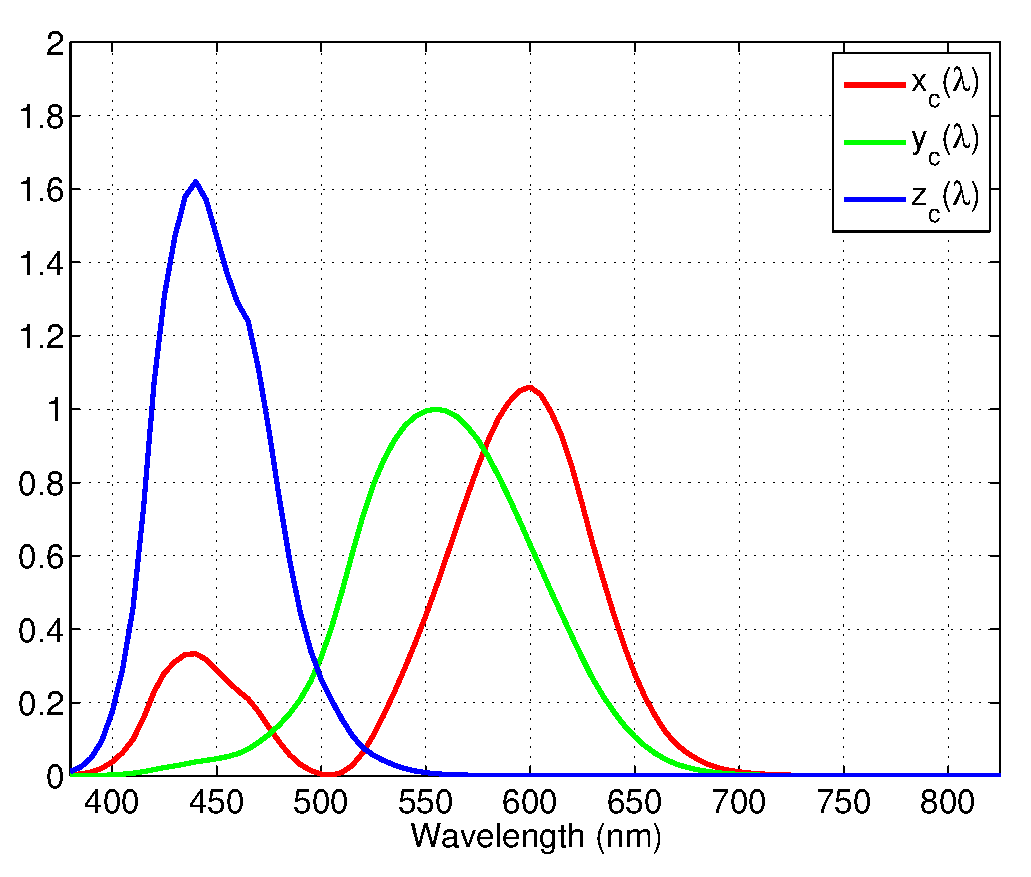
\includegraphics[trim={0.05in 0.05in 0.05in 0.05in}, clip=true, width=2.9in]{img/CIE1931CMF.eps}
	\caption{CIE XYZ 1931 model color matching functions}
	\label{fig:CIE1931CMF}
\end{figure}

The \textit{commission internationale de l'$\acute{e}$clairage} (CIE) specified the CIE 1931 XYZ color space. It maps an SPD to a color representation as sensed by the human eye. The standard defines three color matching functions $x_c(\lambda)$, $y_c(\lambda)$, and $z_c(\lambda)$ as shown in \figurename{ \ref{fig:CIE1931CMF}}. The tristimulus values for the XYZ primaries are given by
\setlength{\arraycolsep}{0.0em}
\begin{subequations}
\begin{align}
X_W &= \int_{\lambda_{min}}^{\lambda_{max}}W(\lambda)x_c(\lambda)d\lambda\\
Y_W &= \int_{\lambda_{min}}^{\lambda_{max}}W(\lambda)y_c(\lambda)d\lambda\\
Z_W &= \int_{\lambda_{min}}^{\lambda_{max}}W(\lambda)z_c(\lambda)d\lambda
\end{align}
\label{eqTriStimulus}
\end{subequations}
\setlength{\arraycolsep}{5pt}

A color can be expressed in terms of its chromaticity and luminance. Chromaticity coordinates capture the hue and saturation of the color while luminance captures the amount of light in the color. The chromaticity coordinates for the SPD can be then be computed from the tristimulus values as
\begin{equation}
\label{eqChromaticity}
	\vecttwo{x}{y} = \frac{1}{X_W+Y_W+Z_W}\vecttwo{X_W}{Y_W}
\end{equation}

The spectral radiance of a black body heated to temperature $T$ as stated by Planck's law is given by
\begin{equation}
\label{eqPlanck}
	 S(\lambda) = \frac{2hc^2}{\lambda^5\left[\text{exp}\left(\frac{hc}{\lambda kT}\right)-1\right]}
\end{equation}
where $h$ is the Planck's constant, $c$ is speed of light, and $k$ is Boltzmann's constant. Replacing $W(\lambda)=S(\lambda)$ in Eq.(\ref{eqTriStimulus}) and then from Eq.(\ref{eqChromaticity}) we obtain the CIE 1931 XYZ chromaticity values $[x,y]$ associated with a black body heated to temperature $T$. In this context $T$ is also known as the CCT for color represented by $[x,y]$. Note that two different SPDs can generate the same chromaticity coordinates. This is due to the principle of metamerism.

Traditionally luminaires have been specified to generate a certain CCT with colors at lower temperature appearing (ironically) warmer than those at higher temperatures. It is practical to generate colors off the black body radiation curve using different colored sources. This analysis considers only the colors generated on the black body radiation curve. As the CCT changes from a lower value to a higher value, the optical power available to transmit information on any color channel varies thus affecting the overall communication performance.

Optical filters can be manufactured to permit narrow-bandpass filtering using plasmonics \cite{xu10a,yok12a}. Broad-bandpass optical filters that make use of interference are widely available. The transmittance of these filters can be modeled as Lorentzian functions of wavelength. The choice of the filter FWHM is a tradeoff to collect the maximum signal while rejecting interference and background illumination.

Responsivity of the receiving elements also affects the aggregate system performance. It depends on the quantum efficiency of the material of sensor. Reference \cite{gha12a} computes responsivity as
\begin{equation}
\label{eqResponsivity}
	 R(\lambda) = \frac{\xi\lambda}{1240}
\end{equation}
where $\xi$ is the quantum efficiency of the material, and $\lambda$ is wavelength of interest. For equal signal radiant flux, signals that span wavelength ranges with lower responsivity will perform poorly as compared to the rest. 

Optical spectrum outside the visible range like infrared (IR) and ultraviolet (UV) spectrum can also be utilized for WDM. It can be seen from \figurename{\ref{fig:CIE1931CMF}} that IR and UV do not generate chromatic response on human eye and thus do not contribute to visible illumination. Thus, as long as their emissions satisfy eye and skin safety regulations, using this additional optical spectrum can only boost the channel capacity.

% Simultion
\section{Simulation}\label{sec:simulation}
Simulations are performed to study how the choice of design parameters like illumination CCT, transmitter SPD, and filter FWHM affect the performance of a multi-wavelength VLC system. Three transmitting elements with Gaussian emission spectrum at dominant wavelengths of red (627 nm), green (530 nm) and blue (470 nm) are selected. Using these transmitting elements, CCT range of [2500 7000] K is sought. SPD spread within [5 50] nm is considered. \figurename{\ref{fig:LEDSPD}} illustrates normalized SPDs needed to achieve the range of CCTs for transmitting elements with 5 nm spread.

\begin{figure}[!b]
	\centering
		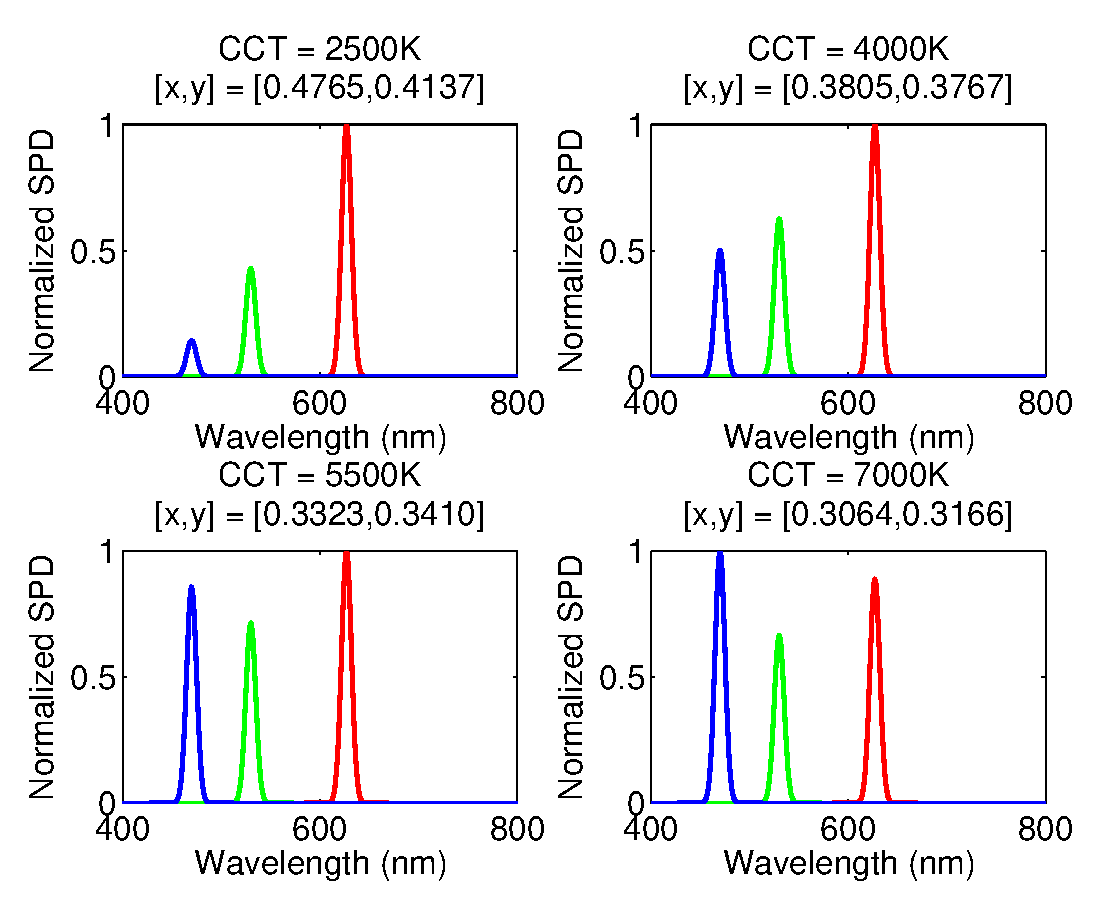
\includegraphics[trim={0.05in 0.05in 0.05in 0.0in}, clip=true, width=2.9in]{img/LEDSPD.eps}
	\caption{Transmitting element normalized spectral power distribution}
	\label{fig:LEDSPD}
\end{figure}

Unique $t_R:t_G:t_B$ ratios are generated after varying the tristimulus values in the range [0 1] in 0.1 unit steps. By substituting these values in Eq.(\ref{eqWhite})-Eq.(\ref{eqChromaticity}), chromaticity coordinates for resulting SPDs are calculated. An initial characterization step generates a pre-populated table consisting of the tristimulus values and corresponding chromaticity coordinates. As the CCT is varied, the chromaticity coordinates are computed as shown in Section \ref{sec:wdm}. From the pre-computed table, the tristimulus values that achieve the closest chromaticity are selected. The SPD is then scaled to achieve target illumination (400 lx) at the receiver that is located at a distance of 2 m from the transmitter. The surface normals of the transmitter and receiver are assumed to be parallel.

\begin{figure}[!t]
	\centering
		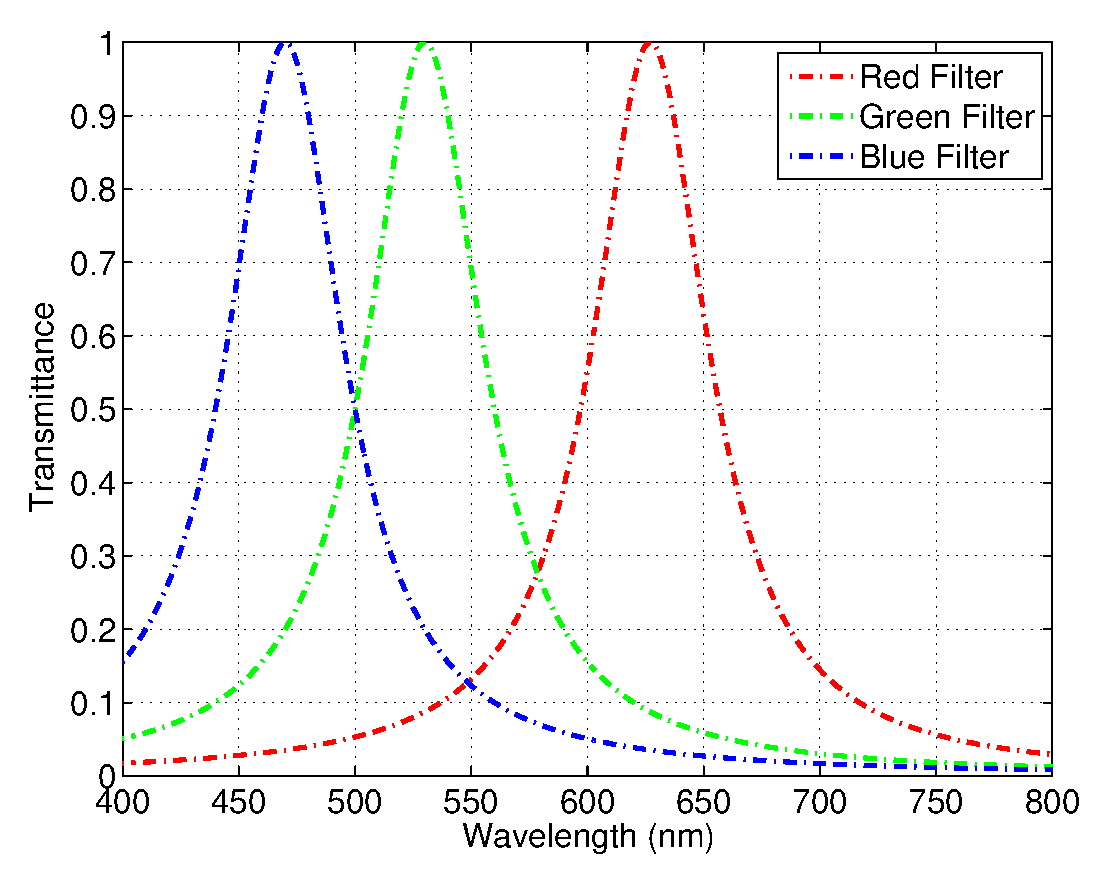
\includegraphics[trim={0.15in 0.05in 0.05in 0.35in}, clip=true, width=2.9in]{img/FiltTr.eps}
	\caption{Filter transmittance for full width at half maximum = 40nm}
	\label{fig:FiltTr}
\end{figure}

Optical filter's passband can be designed to center on the transmitting elements' dominant wavelengths. Optical filters for the simulation are modeled to have Lorentzian transmittance with ideal value $1$ at the dominant red, green and blue wavelengths mentioned above. Filter transmittance as a function of wavelength is illustrated in \figurename{\ref{fig:FiltTr}}. Filter FWHM considered for the analysis lie in [1 250] nm range.

The receiver sensor is assumed to be made of silicon. The assumed quantum efficiencies and responsivity of the sensor taken from source \cite{qeff} is illustrated in \figurename{\ref{fig:RecvResp}}. The responsivity near the blue wavelength is about 0.29 A.W$^{-1}$ and increases steadily to about 0.46 A.W$^{-1}$ near the red before rapidly reducing as the energy of the incident photon approaches the bandgap energy of silicon.

To analyze the system performance with reasonable number of iterations, transmitting and receiving elements are restricted to the same deviations about their respective means. A random bit stream is then generated. Bits for each link are then using asymmetrically clipped offset and DC-biased optical orthogonal frequency division multiplexing (ACO-OFDM and DCO-OFDM). Details on these optical OFDM techniques can be found in references \cite{car96a,arm06a}. For this simulation, ACO-OFDM and DCO-OFDM are implemented with 64 sub-carriers and 64-QAM and 8-QAM modulation, respectively. This ensures that both schemes achieve similar bits/symbol with ACO-OFDM achieving 96 bits/symbol and DCO-OFDM achieving 93 bits/symbol. The DC level on each link is set to ensure the desired CCT is achieved at the 400 lx illumination level. This generates the transmit vector $\vm{X}$. 

\begin{figure}[!b]
	\centering
		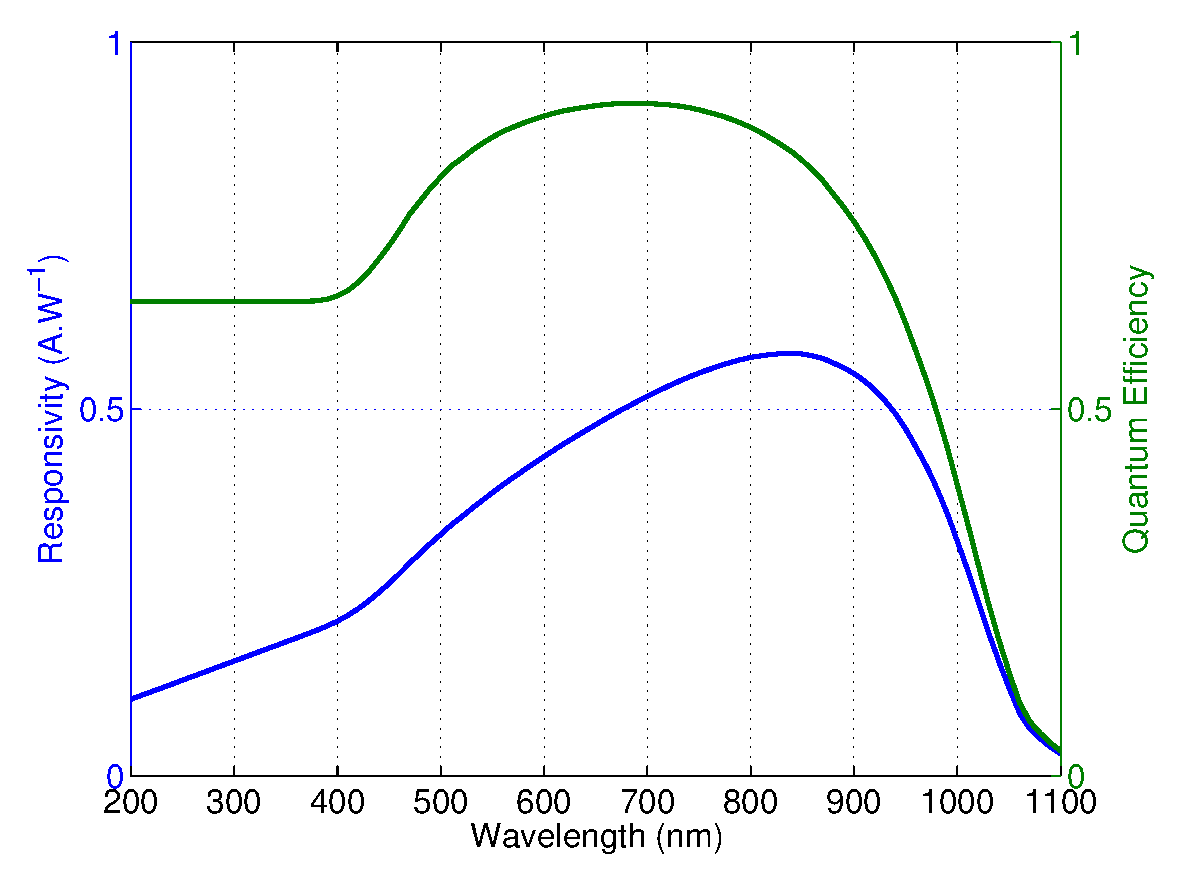
\includegraphics[trim={0.15in 0.05in 0.05in 0.0in}, clip=true, width=2.9in]{img/RecvResp.eps}
	\caption{Receiver quantum efficiency and responsivity \cite{qeff}}
	\label{fig:RecvResp}
\end{figure}

\begin{figure*}[tbph]
\centerline{\subfloat[Most power efficient operation point]{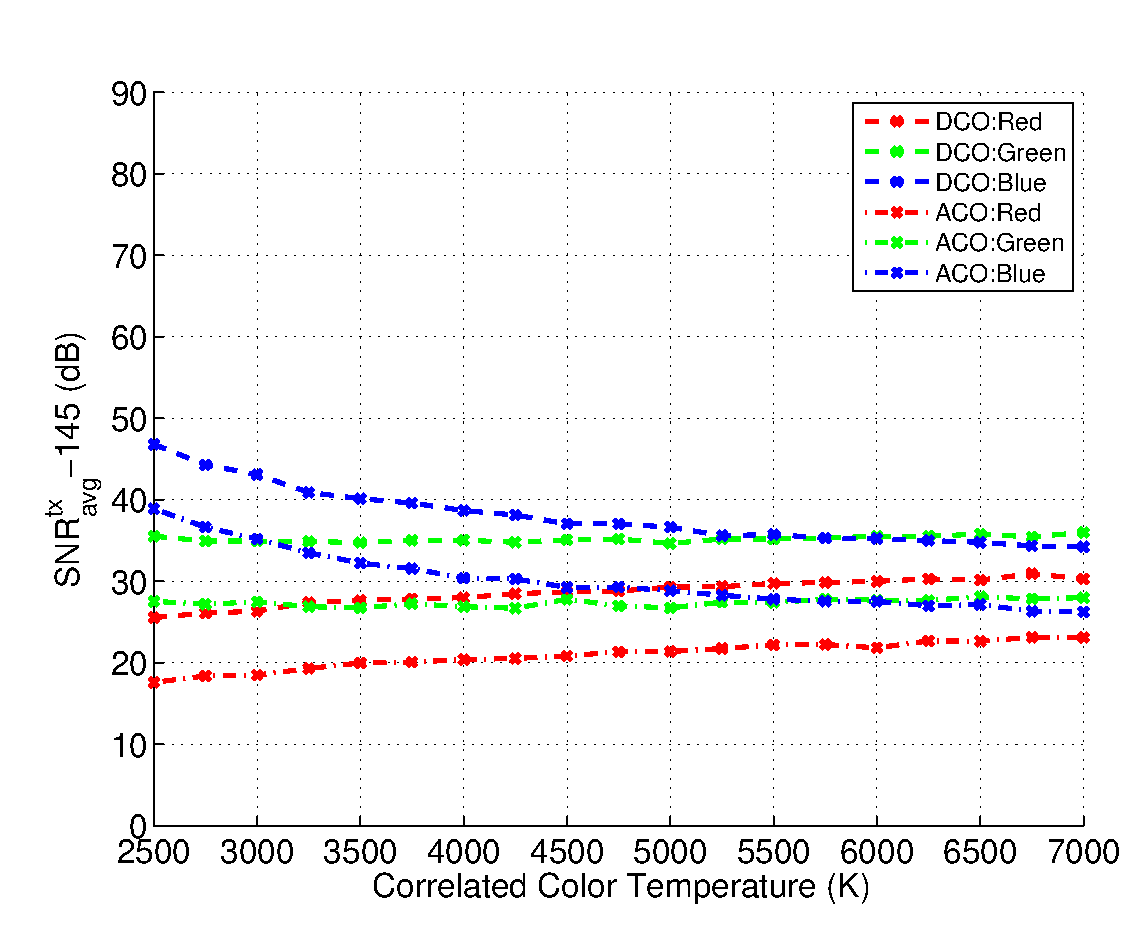
\includegraphics[trim={0.15in 0.05in 0.05in 0.35in}, clip=true, width=2.9in]{img/SNRvsCCT.eps} \label{subfig:SNRvsCCThigh}}
\hfil 
\subfloat[High inter-channel interference]{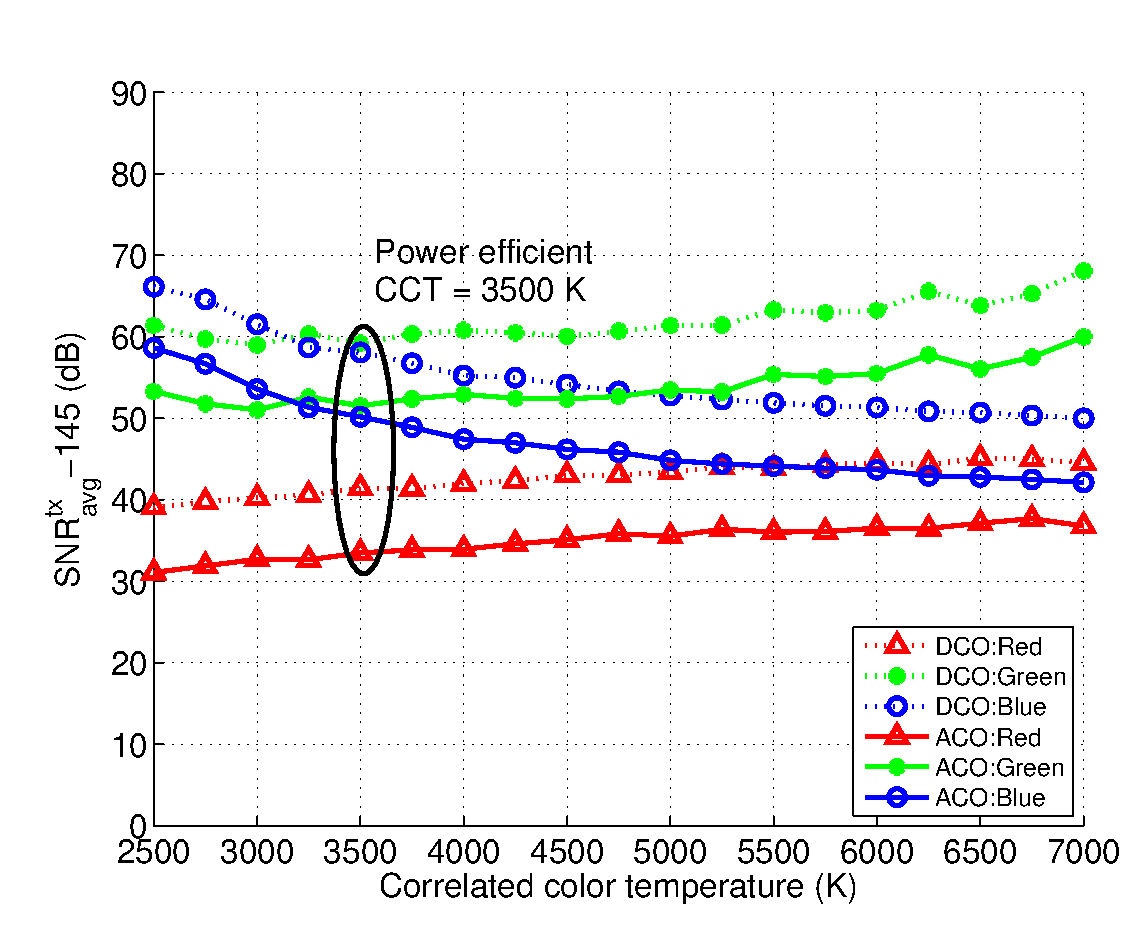
\includegraphics[trim={0.15in 0.05in 0.05in 0.35in}, clip=true, width=2.9in]{img/SNRvsCCT2.eps} \label{subfig:SNRvsCCTlow}}}
\caption{$\text{SNR}^{\text{tx}}_{\text{avg}}$ vs correlated color temperature to achieve BER $\leq 10^{-3}$ \newline(a) Transmitter: $\sigma_r = \sigma_g = \sigma_b = 5$ nm; Filter: $\Gamma_r = \Gamma_g = \Gamma_b = 40$ nm (b) Transmitter: $\sigma_r = \sigma_g = \sigma_b = 50$ nm; Filter: $\Gamma_r = \Gamma_g = \Gamma_b = 250$ nm}
\label{fig:SNRvsCCT}
\end{figure*}
\global\let\figone\relax

Having established $N_{tx} = 3$ transmitting and $N_{rx} = 3$ receiving elements, the $3\times 3$ channel matrix $\vm{H}$ can be computed as in Section \ref{sec:mimo}. AWGN vector $\vm{W}$ is generated and is then added to the transmitted vector. With the knowledge of the transmitted signal power and by varying the receiver noise, simulations over a range of $\text{SNR}^{\text{tx}}_{\text{avg}}$ are carried out. Vector \vm{Y} then collects the received signal and the added noise and interference. The least squares estimate of the transmitted signal vector is computed as
\begin{equation}
	\label{eqXhat}
	\hat{\vm{X}} = (\vm{H}^{*}\vm{H})^{-1}\vm{H}^{*}\vm{Y}
\end{equation}
An estimate of the transmitted optical OFDM frame for each color is obtained by aggregating least squares estimates of the received signal vectors. Further signal processing on each optical OFDM frame gets an estimate of the transmitted QAM symbol. Decoding the QAM symbols provides an estimate of the transmitted bits. Bit error rate (BER) is then calculated by comparing the transmit and estimated bit streams.


% Results
\section{Simulation and Results}\label{sec:results}
We wish to study how the choice of design parameters like transmitter SPD, filter transmittance and CCT affect the performance of a multi-colored VLC system. We chose three transmitting elements with dominant wavelengths at red (627 nm), green (530 nm) and blue (470 nm). These are modeled to have Gaussian emission spectrum. We also seek to achieve CCT range of [2500 7000] K. Normalized SPDs to achieve this range of CCTs with different transmitting SPD widths is illustrated in {\color{red}figure}. For all CCTs, a total received illumination of 400 lx is maintained. 

Unique $t_R:t_G:t_B$ ratios are generated after varying the tristimulus values in the range [0 1] in 0.1 unit steps. By substituting these values in Eq.(\ref{eqWhite})-Eq.(\ref{eqChromaticity}), we calculate chromaticity coordinates for resulting SPDs. An initial characterization step generates a pre-populated table consisting of the tristimulus values and corresponding chromaticity coordinates. As the CCT is varied, the chromaticity coordinates are computed as shown in Section \ref{sec:wdm}. From the pre-computed table, the tristimulus values that achieve the closest chromaticity are selected. The SPD is then scaled to achieve target illumination (400 lx) at the receiver. 

Optical filter's passband can be designed to center on the transmitting element's dominant wavelength. Optical filters for the simulation are modeled to have Lorentzian transmittance with ideal value $1$ at the dominant red, green and blue wavelengths mentioned above. Filter transmittance as a function of wavelength is illustrated in {\color{red}figure}. Filter FWHM considered for the analysis lie in [1 150] nm range.

We assume the receiver sensor to be made of silicon. The assumed quantum efficiencies and responsivity of the sensor is illustrated in {\color{red}figure}. The responsivity near the blue wavelength is about {\color{red}0.1 A.W$^{-1}$} and increases steadily to about {\color{red}0.4 A.W$^{-1}$} near the red before rapidly reducing as the energy of the incident photon approaches the bandgap energy of silicon.

Having established $N_{tx} = 3$ transmitting and $N_{rx} = 3$ receiving elements, the $3\times 3$ channel matrix $\vm{H}$ can be computed as in Section \ref{sec:mimo}. To analyze the system performance, a random bit stream is generated. Bits for each link are then framed using ACO-OFDM and DCO-OFDM using 64 sub-carriers and 64-QAM and 32-QAM modulation respectively. The DC level on each link is set to ensure the desired CCT is achieved at the illumination levels. This generates the transmit vector $\vm{X}$. Noise is then added to the transmitted vector. \vm{Y} then collects the received signal and the added noise and interference. The signal is estimated and decoded. Bit error rate (BER) is then calculated by comparing the transmit and estimated bit streams.

The change in performance of the red, green and blue links as the CCT is varied is shown in {\color{red}figure}. At 2500K, the SPD has a greater contribution from red, then green and then blue. Thus the red link achieves target BER at lower signal power. As the CCT increases from 2500K to 7000K, the red signal power decreases, green signal power remains similar and the blue signal power increases. The performance of the red link starts degrading, while that of the green remains relatively unchanged while that of the blue improves with increase in CCT.

The change in performance of the red, green and blue links as the transmitting element SPD width is varied is shown in {\color{red}figure}. As the SPD width is increased, the performance of all three links degrade. This can be attributed to two factors. Initially, as the signal power is distributed across a larger wavelength range, with the filter transmittance function remaining the same, increasingly more signal gets rejected by the filter. This the receiver collects a smaller fraction of the signal power, degrading the performance. Secondly, as the individual SPDs become wide enough, they start overlapping and causing ICI. The effect of ICI is more pronounced on the green channel because it gets interference from both, red and blue. Thus transmitting elements with narrower emission spectra perform better.

The change in performance of the red, green and blue links as the receiving element filter FWHM is varied is shown in {\color{red}figure}. As the filter FWHM is increased from 0 nm to 250 nm, initially the system performance improves with the best performance for each link within the 40 nm - 80 nm range. At the lower FWHM ranges, the filters transmit a smaller fraction of the signal to the sensors and thus performance is limited by the amount of signal power collected for each link. At higher FWHM ranges, along with additional signal, the filters permit increasingly more ambient light and signals from neighboring channels. This adds additional noise and interference to the link, thus degrading the performance. For the specified multi-colored system, filter FWHM within [40 80]nm seems optimal.

\begin{figure}
	\centering
		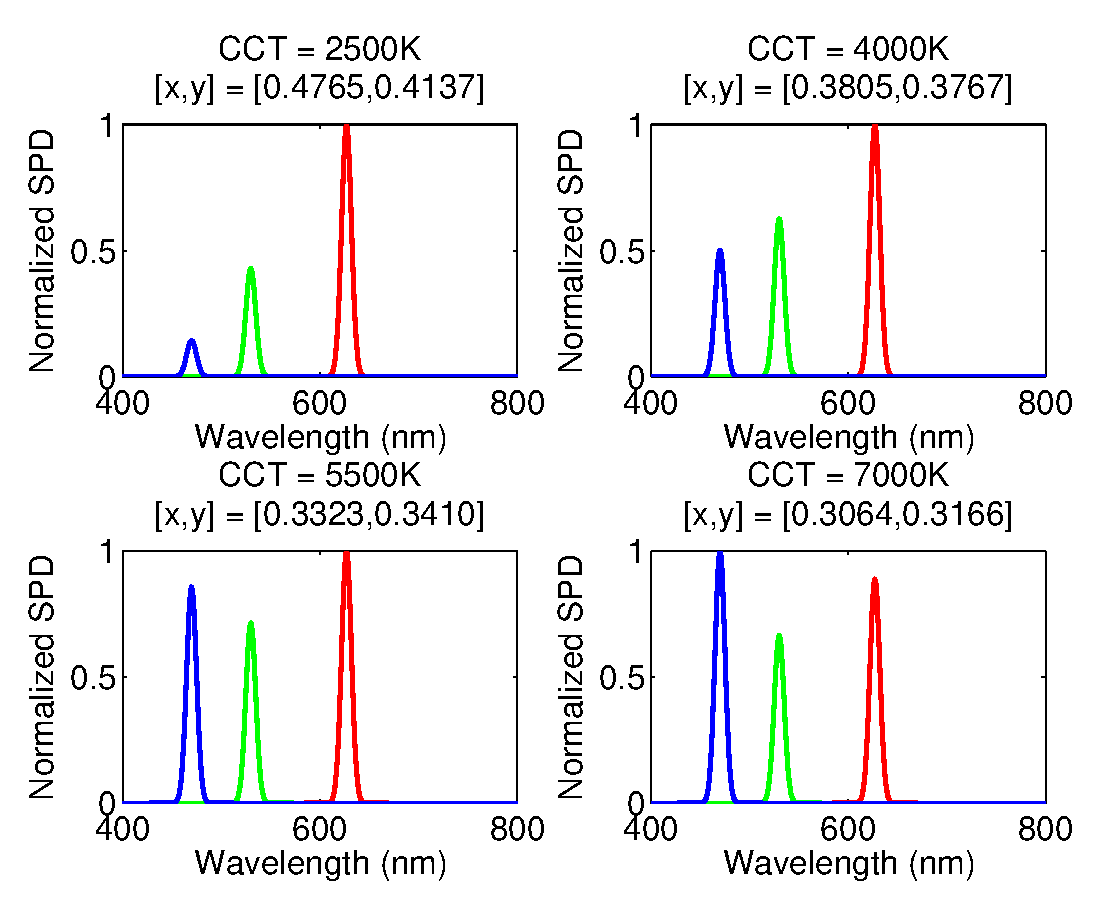
\includegraphics[width=3in]{img/LEDSPD.eps}
	\caption{Transmitting Element Normalized Spectral Power Distribution}
	\label{fig:LEDSPD}
\end{figure}

\begin{figure}
	\centering
		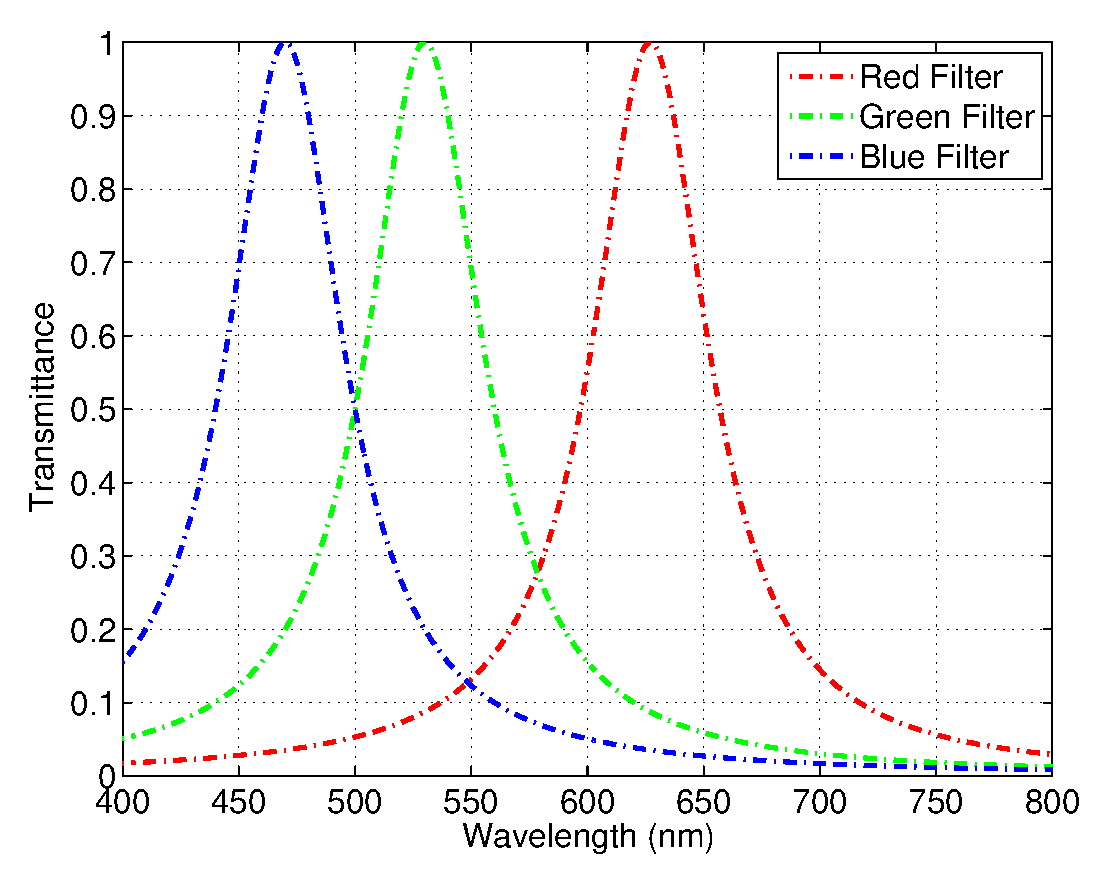
\includegraphics[width=3in]{img/FiltTr.eps}
	\caption{Filter Transmittance (FWHM=60nm)}
	\label{fig:FiltTr}
\end{figure}

\begin{figure}
	\centering
		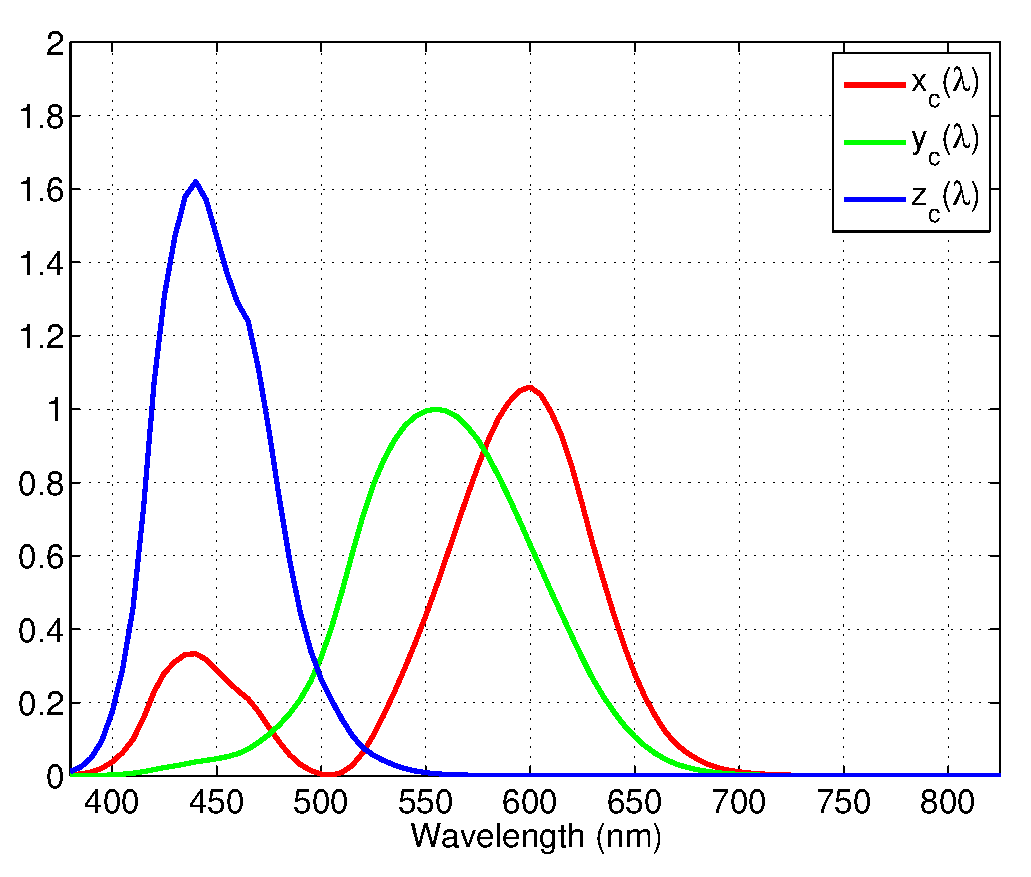
\includegraphics[width=3in]{img/CIE1931CMF.eps}
	\caption{CIE XYZ 1931 Model Color Matching Functions}
	\label{fig:CIE1931CMF}
\end{figure}

\begin{figure}
	\centering
		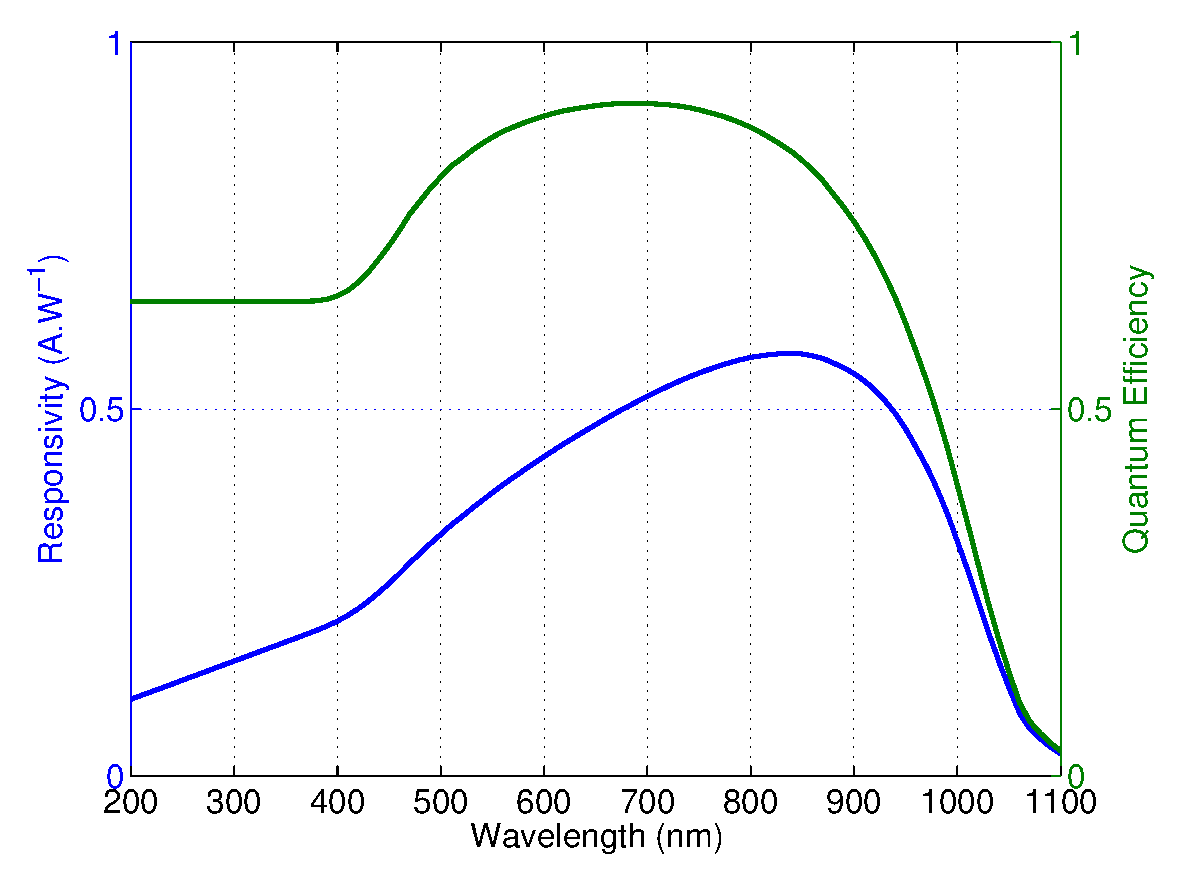
\includegraphics[width=3in]{img/RecvResp.eps}
	\caption{Receiver Responsivity}
	\label{fig:RecvResp}
\end{figure}

\begin{figure}
	\centering
		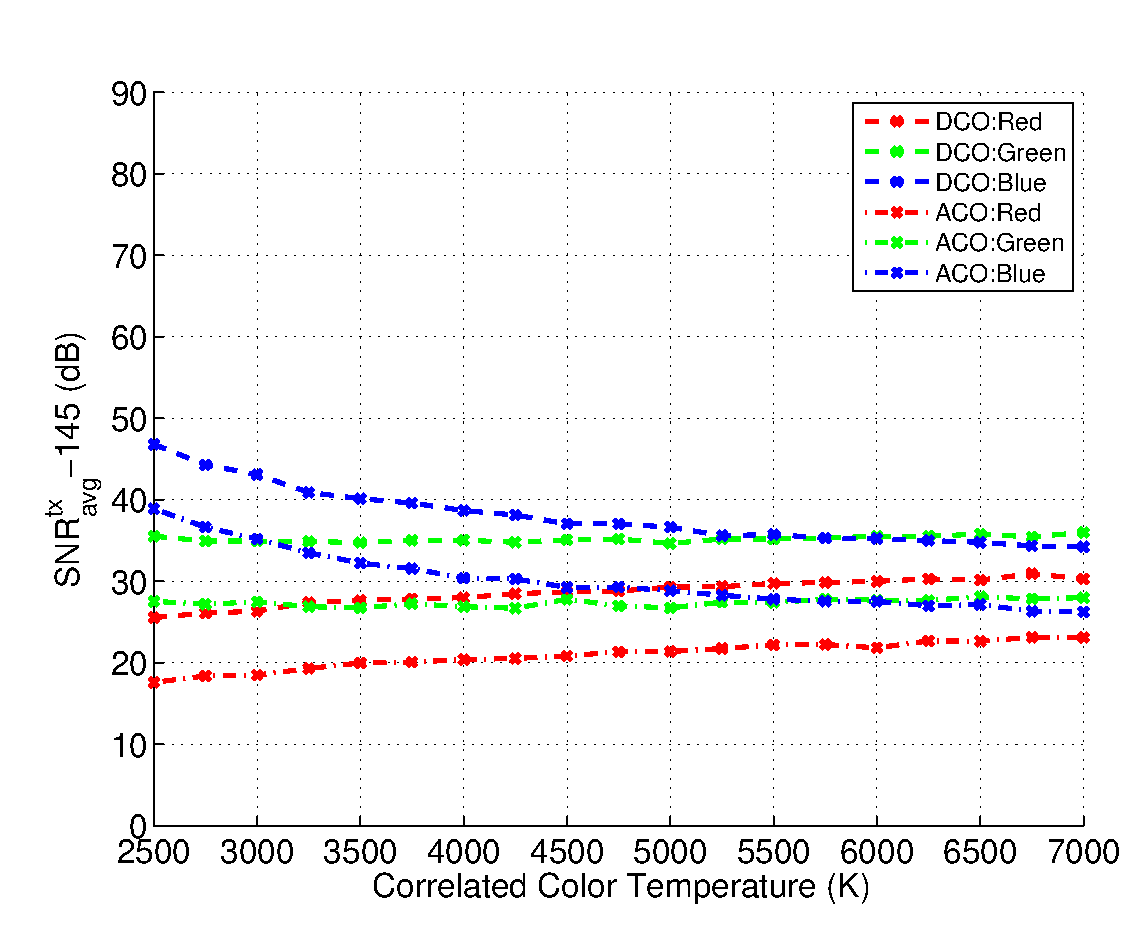
\includegraphics[width=3in]{img/SNRvsCCT.eps}
	\caption{$SNR_{avg}^{tx}$ vs Corelated Color Temperature}
	\label{fig:SNRvsCCT}
\end{figure}

\begin{figure}
	\centering
		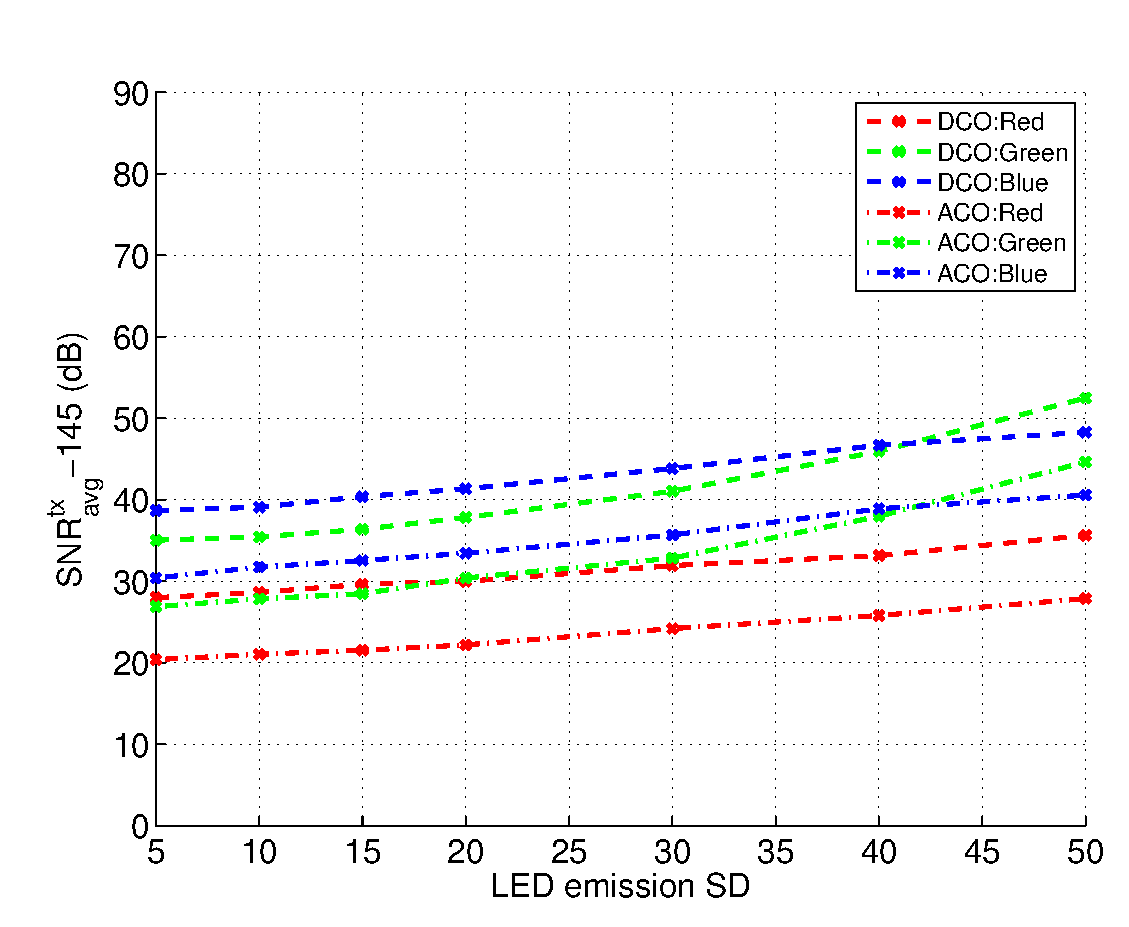
\includegraphics[width=3in]{img/SNRvsLEDSD.eps}
	\caption{$SNR_{avg}^{tx}$ vs Transmitting Element Spectral Power Distribution Width}
	\label{fig:SNRvsLEDSD}
\end{figure}

\begin{figure}
	\centering
		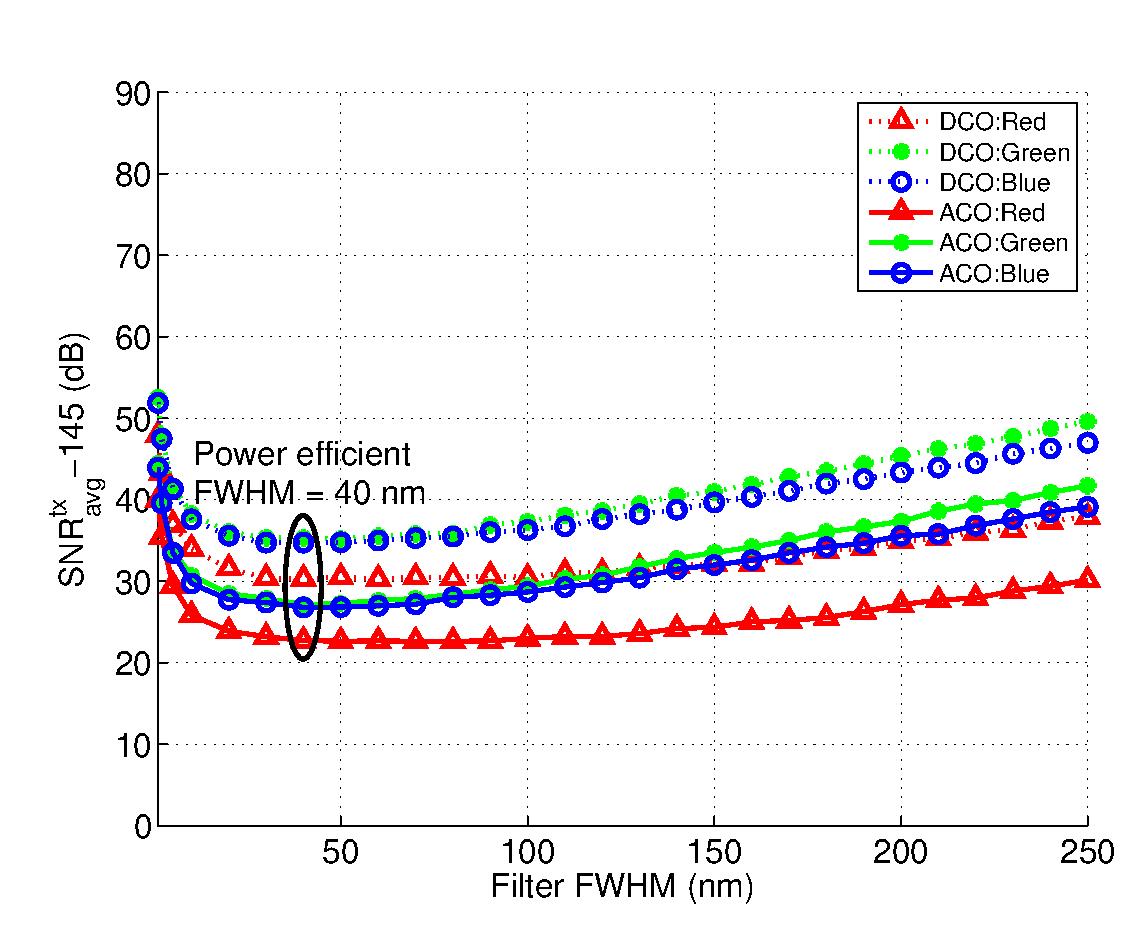
\includegraphics[width=3in]{img/SNRvsFLTWID.eps}
	\caption{$SNR_{avg}^{tx}$ vs Filter Full Width at Half Maximum}
	\label{fig:SNRvsFLTWID}
\end{figure}










% Conclusion
\section{Conclusion}\label{sec:conclusion}
In this work, multi-wavelength VLC system in the context of variable illumination constraints was introduced. VLC system performance was characterized for variations in illumination CCT, transmitter SPD spread, and the receiver filter transmittance FWHM. For the three colored system considered, the blue and the green links pose the performance bottlenecks because of the relatively lower contribution to the SPD and lower photodiode responsivity as compared to the red. As the ICI increases, the most power efficient CCT shifts towards lower temperatures. Transmitting elements with the smallest spectral spread provide the most power efficient operating point. The effect of increase in spectral spread is most pronounced in the green link because it suffers the most from interference from the blue and red links. Filters with narrow transmittance FWHM reject a lot of the signal power while filters with a broad transmittance FWHM accept a lot of interference. Both of these affect the power efficiency of the system. For the setup considered, least power efficient operating point is for DCO-OFDM at CCT = 2500 K, transmitting element SPD spread = 50 nm, and filter FWHM = 1 nm. The most power efficient operating point is for ACO-OFDM at CCT = 6250 K, transmitting element SPD spread = 5 nm, and filter FWHM = 40 nm.
% Acknowledgement
\section{Acknowledgement}
This work was supported by the Engineering Research Centers Program of the National Science Foundation under NSF Cooperative Agreement No. EEC-0812056.
% Bibliography
\bibliographystyle{IEEEtran}
\bibliography{WDMOFDM}
\end{document}